\subsection{Teilaufgabe 1: Algorithmik}

\subsection{Teilaufgabe 2: Theoretische Informatik}

\subsubsection{Aufgabe 1: Reguläre Sprachen}

\begin{teile}
	\item
	$L_a = \{w \in \Sigma^* | \nexists u,u' \in \Sigma^*: w =u(ab)u'\} = ((b|c)^*(a^*c)^*(b|c)^*)^*a^*$
	
	\textbf{Erklärung}: \\
	Alle Wörter in $L_a$ setzen sich aus Teilworten zusammen, die eine zusammenhängendes Teilwort beliebiger Länge aus $a$'s enthalten. Vor und nach dem $a$-Block dürfen beliebige Wörter aus $b$'s und $c$'s vorkommen (deshalb $(b|c)^*$ in regulären Ausdruck). Sobald ein $a$ erscheint, dürfen weitere $a$'s folgen (deshalb $a^*$ in regulären Ausdruck) oder ein $c$ (deshalb folgt auf $a^*$ immer das $c$, außer am Ende des Wortes). Es müssen auch gar keine $a$'s vorkommen (dehalb sind alle Bestandteile, in denen $a$'s vorkommen, mit $^*$ versehen).

	\item
	$L_b = L(M) = a^*|(a^* ba^* ba^* ba^* ba^*)^*$.
	
	\textbf{Begründung}: \\
	Anfangs befinden wir uns in einem Endzustand, der beliebig viele weitere $a$'s zulässt (deshalb $a^*$ in regulären Ausdruck).\\
	Verlässt man diesen Endzustand über ein $b$, muss ein Zyklus mit genau vier $b$'s durchlaufen werden, zwischen denen jeweils beliebig viele $a$'s liegen dürfen, bevor wieder der Endzustand erreicht wird (deshalb $a^* ba^* ba^* ba^* ba^*$ in regulären Ausdruck). Dieser Zyklus kann beliebig oft durchlaufen werden (deshalb das $^*$ bei der rechten Klammer im regulären Ausdruck).
	
	\item	
	Zur besseren Übersicht wird zunächst die \textbf{Zustandsübergangs-Tabelle} des Automaten aufgestellt:\\
	\begin{tabular}{|c|c|c|}
		\hline
		\textbf{Zustand} & \textbf{0} & \textbf{1} \\
		\hline
		0                & 1          & 3 \\
		\hline
		1                & 0          & 6 \\
		\hline
		2                & 1          & 4 \\
		\hline
		3                & 4          & 4 \\
		\hline
		4                & 4          & 5 \\
		\hline
		5                & 0          & 5 \\
		\hline
		6                & 0          & 5 \\
		\hline
	\end{tabular} 
	
	Um die Erreichbarkeit aller Zustände zu überprüfen wird eine \textbf{Zeugentabelle} angefertigt:\\
	\begin{tabular}{l|ccccccc}
		\textbf{Zustand} & 0          & 1 & 2 & 3 & 4  & 5   & 6 \\
		\hline
		\textbf{Zeuge}   & $\epsilon$ & 0 & - & 1 & 11 & 111 & 01 \\
	\end{tabular} 
	Zustand 2 ist also nicht erreichbar, deshalb entfällt er im minimierten Automaten.
	
	Nun wird das bekannte \textbf{Tabellenfüllverfahren} zur Bestimmung äquivalenter Zustände durchgeführt: 
	
	\includegraphics[scale=0.7]{Tabellenfüllverfahren.png}

	Da Zusatnd 4 der einzige Endzustand ist, werden zunächst alle Zustandspaare in der Tabelle, die 4 und einen weiteren Zustand enthalten, mit $X_0$ markiert.
	
	Die weiteren Markierungen in der Tabelle gehen aus folgender Tabelle hervor, welche die Übergänge der Zustandspaare angibt:

	\begin{tabular}{c|c|c|l}
		\textbf{Zustandspaar} & \textbf{0} & \textbf{1} & \textbf{Erläuterung} \\
		\hline
		(0,1)                 & (0,1)      & (3,6)      & Eingabe 1: (3,6) führt zu X3. Ergänze X5. \\		
		\hline
		(0,3)                 & (1,4)      & (3,4)      & Eingabe 0: (1,4) führt zu X0. Ergänze X1. \\
		\hline
		(1,3)                 & (0,4)      & (4,6)      & Eingabe 0: (0,4) führt zu X0. Ergänze X4. \\
		\hline 		 		
		(0,5)                 & (0,1)      & (3,5)      & Eingabe 0: (3,5) führt zu X2. Ergänze X6. \\
		\hline 		
		(1,5)                 & (0,0)      & (5,6)      & \\
		\hline
		(3,5)                 & (0,4)      & (4,5)      & Eingabe 0: (0,4) führt zu X0. Ergänze X2. \\
		\hline
		(0,6)                 & (0,1)      & (3,5)      & Eingabe 1: (3,5) führt zu X2. Ergänze X7. \\
		\hline
		(1,6)                 & (0,0)      & (5,6)      & \\
		\hline
		(3,6)                 & (0,4)      & (4,5)      & Eingabe 0: (0,4) führt zu X0. Ergänze X3. \\
		\hline
		(6,5)                 & (0,0)      & (5,5)      & \\
	\end{tabular} 
	
	Die Zuständspaare 1, 5 und 6 bleiben nach wiederholtem Durchlaufen und Überprüfen unmarkiert. Folglich liegen 1, 5 und 6 in der selben Äquivalentsklasse und bilden im minimietern Automaten den Zustand $[1,5,6]$. Insgesamt ergeben sich also folgende Äquivalenzklassen als Zustände für den minimierten Automaten: $[0],[1,5,6],[3],[4]$
	
	Der minimierte Automat $A'$ sieht also folgendermaßen aus: \\
	$A' = (\{[0],[1,5,6],[3],[4] \},\{0,1\},\delta, [0], \{[4]\})$

	\begin{figure}[ht]
		\begin{minipage}[t]{.4\textwidth}
			\hspace*{25pt}
			mit $\delta$:

			\hspace*{25pt}
			\begin{tabular}{|l|l|l|}
				\hline
				\textbf{Zustand} & \textbf{0} & \textbf{1} \\
				\hline
				[0]            & [1,5,6]    & [3] \\ 
				\hline
				[1,5,6]        & [0]        & [1,5,6] \\
				\hline
				[3]            & [4]        & [4] \\
				\hline  
				[4]            & [4]        & [1,5,6] \\
				\hline 
			\end{tabular}
		\end{minipage}
		\begin{minipage}[t]{.57\textwidth}
			\vspace*{0pt}
			\hspace*{20pt}
			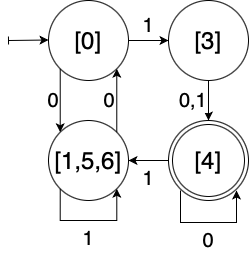
\includegraphics[scale=0.35]{DEA_T1_A1.png}
		\end{minipage} 
	\end{figure}
	
\end{teile}

\newpage
\subsubsection{Aufgabe 2: Kontextfreie Sprachen}

\begin{teile}
	\item
	Ja, das Wort \glqq abba\grqq\ ist mit $G$ ableitbar und liegt somit in $L(G)$, wie mit dem CYK-Algorithmus nachgewiesen werden kann:
	
	\begin{center}
		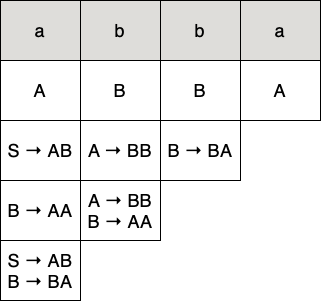
\includegraphics[scale=0.45]{CYK-Pyramide.png}
	\end{center}
	
	Der Ableitungsbaum lässt sich aus der Tabelle ablesen:
	
	\begin{center}
		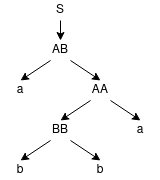
\includegraphics[scale=0.7]{Ableitungsbaum.png}
	\end{center}
		
	\item
	\begin{enumerate}[label=\roman*.]
		\item
		Es gilt: $K\cdot R = \{k\circ r\ |\ \forall k \in K, r \in R\}$

		Die regulären Sprachen sind eine Teilmenge der kontextfreien Sprachen.
		Also ist auch $R$ kontextfrei. Kontextfreie Sprachen sind abgeschlossen unter \emph{Verkettung}: \\
		Sei $G_1 = (N_1, \Sigma_1, P_1, S_1)$ die kontextfreie Grammatik, welche $K$ erzeugt, und $G_2 = (N_2, \Sigma_2, P_2, S_2)$ die kontextfreie Grammatik, welche $R$ erzeugt. Dann kann eine kontextfreie Grammatik $G$ konstruiert werden, welche die Verkettung von $K$ und $R$ erzeugt:\\
		Man ergänze dafür ein neues Startsymbol $S$, sowie eine neue Produktionsregel $S \rightarrow S_1S_2$ und erhält $G = (N_1 \cup N_2 \cup \{S\}, \Sigma_1 \cup \Sigma_2, P_1 \cup P_2 \cup \{S \rightarrow S_1S_2\}, S)$.\\
		Da $L(G)=K\cdot R$ ist diese Sprache kontextfrei.

		Die Aussage ist also wahr.
				
		\item
		$L'$ ist bekanntermaßen nicht kontextfrei. Die Sprache $K = \{a^n\ |\ n \in \mathbb{N}_0\}$ über dem Alphabet $\Sigma = \{a,b,c\}$ ist regulär - denn es gilt $K = a^*$, also gibt es einen regulären Ausdruck für $K$ - und somit auch kontextfrei.\\
		Allerdings gilt auch für $K \circ L' = \{a^nb^mc^m\ |\ n,m \in \mathbb{N}_0\}$, das die Sprache regulär, mit Ausdruck: $K \circ L'= a^*(bc)^*$, und somit kontextfrei ist.
		
		Dieses Gegenbeispiel beweist, dass die Aussage falsch ist.
		
	\end{enumerate}
	
	
\end{teile}

\newpage
\subsubsection{Aufgabe 3: Chomsky-Hierarchie}

\begin{teile}
	\item
	$L_1 = \{ w \in L: vor\ jedem\ (\ stehen\ mehr\ [\ als\ ] \}$ 
	
	\begin{quote}
		\textbf{Pumpinglemma für kontextfreie Sprachen} \\
		Ist $L$ eine kontextfreie Sprache, so gilt: \\
		$\exists p \in \mathbb{N}: \forall z \in L, |z| \geq p:$ \\
		$\exists u,v,w,x,y \in \Sigma^*: z = uvwxy$ mit
		\begin{enumerate}
			\item $|vx| \geq 1$
			\item $|vwx| \leq p$
			\item $\forall i \in \mathbb{N} : uv^{i}wx^{i}y \in L$
		\end{enumerate}
	\end{quote}

	Nehmen wir an $L_1$ sei kontextfrei, dann können wir das Pumpinglemma anwenden und folgern:
	
	Sei $p \in \mathbb{N}$ die Pumpingzahl. Wir wählen $z = [^p(]^p)] \in L_1$ mit $|z| = 2p+2 > p$.\\
	Aus $|vwx| \leq p$ und $|vx| \geq 1$ ergeben sich für die Form von $vwx$ folgende Fälle:
	\begin{enumerate}
		\item $v=[^k$ und $x=[^l$ mit $p \geq k+l  \geq 1$
		\item $v=[^k$ und $x=[^l(]^m$ mit $p-1 \geq k+l+m  \geq 0$
		\item $v=[^k(]^l$ und $x=]^m$ mit $p-1 \geq k+l+m  \geq 0$
		\item $v=]^l$ und $x=]^m$ mit $p \geq l+m  \geq 1$
		\item $v=]^l$ und $x=]^m)$ mit $p-1 \geq l+m  \geq 0$
	\end{enumerate}

	In Fall 1 ist $uv^2wx^2y=[^{p+k+l}(]^{p}) \notin L_1$, da $p+k+l > p$ und somit liegt keine korrekte Klammerung mehr vor.\\
	In Fall 2 ist $uv^2wx^2y=[^{p+k}(]^{m}[^{l}(]^{p}) \notin L_1$, da zwei $($ und nur eine $)$ vorkommen. Somit liegt keine korrekte Klammerung vor.\\
	In Fall 3 ist $uv^2wx^2y=[^{p}(]^{l}[^{k}(]^{p+m}) \notin L_1$, da zwei $($ und nur eine $)$ vorkommen. Somit liegt keine korrekte Klammerung vor.\\
	In Fall 4 ist $uv^2wx^2y=[^{p}(]^{p+l+m}) \notin L_1$, da $p+l+m > p$ und somit liegt keine korrekte Klammerung mehr vor.\\
	In Fall 5 ist $uv^2wx^2y=[^{p}(]^{p+l})]^{m}) \notin L_1$, da zwei $)$ und nur eine $($ vorkommen. Somit liegt keine korrekte Klammerung vor.
	
	Das ist ein Widerspruch zur Annahme $L_1$ sei kontextfrei. $\Rightarrow L_1$ ist nicht kontextfrei $\Rightarrow L_1$ ist nicht regulär, da die regulären Sprachen eine Teilmenge der kontextfreien Sprachen bilden. 

	\vspace{0.3cm}
	\item 
	$L_2 = \{ w \in L: auf\ jede\ \ddot{o}ffnende\ Klammer\ folgt\ direkt\ eine\ schließende\ Klammer \}$
	
	Zu $L_2$ lässt sich folgender DEA bauen, der sie akzeptiert:
	\begin{center}
		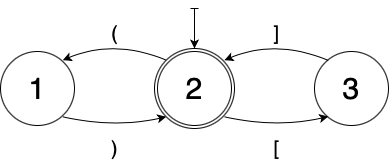
\includegraphics[scale=0.5]{DEA zu Klammersprache.png}	
	\end{center}
	
	Somit ist $L_2$ regulär und damit auch kontextfrei, denn die regulären Sprachen sind eine Teilmenge der kontextfreien Sprachen.
	
\end{teile}

\newpage
\subsubsection{Aufgabe 4: Entscheidbarkeit}

\begin{teile}
 
	\item 
	$L_{1}$ ist nicht entscheidbar.

	TODO

	Angenommen, $L_{1}$ wäre entscheidbar. Dann gäbe es eine Turingmaschine $D$, die für jede Eingabe $\langle M \rangle$ entscheiden kann, ob $M$ auf $\langle N \rangle$ hält und dafür mindestens $2^{|\langle N \rangle|}$ Schritte benötigt. Dies würde bedeuten, dass $D$ die Laufzeit von $M$ auf $\langle N \rangle$ berechnen kann. 

	Allerdings ist bekannt, dass das Halteproblem unentscheidbar ist. Da das Halteproblem unentscheidbar ist, ist auch die Frage, ob $M$ mindestens $2^{|\langle N \rangle|}$ Schritte benötigt, unentscheidbar, da dies eine strengere Bedingung ist, die das Halteproblem als Teilproblem enthält.

	Da $L_{1}$ eine strengere Form des Halteproblems darstellt, muss auch $L_{1}$ unentscheidbar sein.
	
	\begin{tabular}{|l|l|l|}
		\hline
		               & \textbf{Halteproblem} & \textbf{$L_1$} \\
		\hline
		Eingabe        & DTM M und Wort w      & DTM M' \\
		\hline 
		Ja-Instanzen   & M hält auf w          & DTM M' hält auf $\langle N \rangle$ nach $\geq 2^{|\langle N \rangle|}$ Schritten  \\ 
		\hline
		Nein-Instanzen & M hält nicht auf w    & DTM M' hält nicht auf $\langle N \rangle$ nach $\geq 2^{|\langle N \rangle|}$ Schritten \\
		\hline  
	\end{tabular}
	
	\textbf{Beschreibung der Reduktion}
	
	Konstruiere M' wie folgt:
	\begin{itemize}
		\item $Eingabe =  \epsilon$? Dann laufe 100 Schritte ohne das Band zu verändern, kehre zurück zum Ausgangspunkt, und verhalte dich wie M auf w.
		\item $Eingabe \neq \epsilon$? Verhalte dich wie M auf w.
	\end{itemize}
	
	\item 
	$L_{2}$ ist nicht entscheidbar.

	Die Nicht-Entscheidbarkeit von $L_2$ wird durch eine Reduktion auf das bereits als unentscheidbar bekannte allgemeine Halteproblem $L_{halt}=\{\langle M \rangle w | M \text{ ist TM, die auf } w \text{ hält} \}$ nachgewiesen. Dazu wird eine totale und berechenbare Funktion $f$ benötigt, für die $f(w) \in L_2 \Leftrightarrow w \in L_{halt}$ gilt. Sei $f:\Sigma^*\rightarrow \Sigma^*$ definiert über:

	TODO

	$f(w)=\begin{cases}
		\langle M' \rangle &\text{falls $w=\langle M \rangle v$ für TM $M$ und $v \in \Sigma^*$}\\
		\varepsilon &\text{sonst}
	\end{cases}$

	Dabei ist $M'$ eine TM, die auf $\langle N \rangle$ hält, genau dann wenn $M$ auf $v$ hält. Dabei lässt sich $M'$ wie folgt konstruieren:
	\begin{itemize}
		\item Überprüfung der Eingabe $w$. Falls $w \neq \langle N \rangle$ in Endlosschleife laufen.
		\item Ansonsten löschen der Eingabe und schreiben von $v$ aufs Band.
		\item Simulieren von $M$ auf $v$. Falls $M$ auf $w$ hält, hält auch $M'$.
	\end{itemize}

	TODO $\Rightarrow$ siehe Bemerkung\footnote[1]{Gilt das in beide Richtungen oder muss man die getrennt behandeln? Andere Richtung: $M'$ hält auf $\langle N \rangle$ $\rightarrow \langle M' \rangle \langle N \rangle$ als Eingabe.}
	
	Die Funktion $f$ ist offensichtlich total. Außerdem lässt sich $f$ nach dem eben beschriebenen Vorgehen berechnen.

	Es bleibt noch zu zeigen, dass $w \in L_{halt} \Leftrightarrow f(w) \in L_2$ gilt. Dies beweisen folgende Äquivalenzumformungen ($\forall w \in \Sigma^*$):
	\begin{align*}
		w \in L_{halt} \Longleftrightarrow\ &w = \langle M \rangle v \text{ mit TM } M \text{ hält auf } v \\
		\Leftrightarrow\ &f(w) = \langle M' \rangle \text{ mit TM } M' \text{ hält auf } \langle N \rangle \\
		\Leftrightarrow\ &f(w) \in L_2
	\end{align*}

	Somit gilt $L_{halt} \leq L_2$ und da $L_{halt}$ unentscheidbar ist, muss auch $L_2$ unentscheidbar sein.

	
	\item
	$L_3$ ist entscheidbar.

	Da $L(N)=\Sigma^*$ muss $N$ auf jedem $w \in \Sigma^*$ halten, um dieses zu akzeptieren. Folglich ist die Menge der Worte über $\Sigma$, auf denen $N$ nicht hält, die leere Menge. Man kann $L_3$ also umschreiben zu:\\
	$L_3= \{\langle M\rangle | M\ h\ddot{a}lt\ auf\ mindestens\ einem\ w \in \varnothing \}$

	Da es kein solches $w$ gibt, kann es auch kein $M$ geben, welches auf $w$ hält. Folglich ist $L_3 = \varnothing$ und somit regulär und auch entscheidbar. 
	
\end{teile}


\newpage
\subsubsection{Aufgabe 5: Komplexitätstheorie}

\begin{teile}
 
	\item 
	Ein Minimalbeispiel für einen Graphen, der eine Beinahe-3-Färbung aber keine 3-Färbung besitzt, sieht wie folgt aus:

	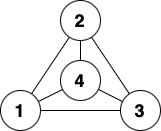
\includegraphics[scale=0.6]{minimal_graph_beinahe-drei-faerbung}
	
	Der Graph besitzt keine 3-Färbung, da Knoten $1,2,3$ und $4$ alle jeweils paarweise durch Kanten verbunden sind. Wenn also Knoten $1,2$ und $3$ mit drei verschiedenen Farben belegt werden, muss für $4$ ebenfalls eine dieser drei Farben gewählt werden und es entsteht eine Kante, die zwei Knoten mit gleicher Farbe verbindet. Folglich besitzt der Graph aber eine Beinahe-3-Färbung.

	\item
	Zunächst werden die genannten Entscheidungsprobleme in formale Sprachen übersetzt:

	$L_{B3F} = \{c(G)\ |\ G=(V,E) \text{ ist Graph, für den eine Beinahe-3-Färbung existiert}\}$

	$L_{3F} = \{c(G)\ |\ G=(V,E) \text{ ist Graph, für den eine 3-Färbung existiert}\}$

	Um zu zeigen, dass das Problem $B3F$ in $\mathcal{NP}$ liegt, wird eine NTM beschrieben, welche $L_{B3F}$ in polynomieller Zeit entscheidet:
	\begin{enumerate}
		\item Durchlaufe den Graphen Knoten für Knoten. ($O(n)$)
		\item Wähle jeweils nichtdeterministisch die passende Farbe, sodass am Ende möglichst wenige Kanten aus zwei gleichfarbigen Knoten entstehen. ($O(1)$)
		\item Gehe alle Kanten durch und überprüfe, ob höchstens eine Kante aus zwei gleichfarbigen Knoten gebildet wird. Wenn das der Fall ist akzeptiere, ansonsten halte und akzeptiere nicht. ($O(n)$)
	\end{enumerate}

	Nun wird eine polynomielle Komplexitäts-Reduktion von $B3F$ auf $3F$ durchgeführt. Dazu wird eine totale und in polynomieller Zeit berechenbare Funktion $f$ benötigt, die Probleme aus $3F$ auf Probleme aus $B3F$ abbildet:

	Sei $f:\Sigma^*\rightarrow \Sigma^*$ definiert über

	$f(w)= \begin{cases}
		c(V\cup \{v_1,v_2,v_3,v_4\}, E\ \cup \{(v_1,v_2),(v_1,v_3), &, falls\ w=c(V,E)\ mit\\
		(v_1,v_4),(v_2,v_3),(v_2,v_4),(v_3,v_4)\}) &\ G = (V,E)\ ist\ Graph\\
		0 &, sonst
	\end{cases}$
	
	$f$ ist offensichtlich total. Außerdem lässt sich eine DTM konstruieren, die $f$ in polynomieller Laufzeit berechnet:
	\begin{itemize}
		\item Syntaxcheck, ob $w=c(V,E)$ mit $e_1,e_2 \in E$ und $G = (V,E)$ ist Graph ($O(n)$).
		\item Passendes anhängen der entsprechenden Knoten und Kanten an Eingabe zu $c(V \cup \{v_1,v_2,v_3,v_4\}, E \cup \{(v_1,v_2),(v_1,v_3),(v_1,v_4),(v_2,v_3),(v_2,v_4),(v_3,v_4)\})$ ($O(n^2)$)
	\end{itemize}

	Es bleibt noch zu zeigen, dass $w \in L_{3F} \Leftrightarrow f(w) \in L_{B3F}$ gilt. Dies beweisen folgende Äquivalenzumformungen ($\forall w \in \Sigma^*$):
	\begin{align*}
		w \in L_{3F} \Longleftrightarrow\ & w=c(V,E)\ mit\ Graph\ G=(V,E)\ besitzt\ eine\ \text{3-Färbung}\\
		\Leftrightarrow\ & f(w)=c(V':=V \cup \{v_1,v_2,v_3,v_4\}, E':=E \cup \{(v_1,v_2),(v_1,v_3),(v_1,v_4),\\
		&\ (v_2,v_3),(v_2,v_4),(v_3,v_4)\})\ mit\ Graph\ G=(V,E)\ besitzt\ eine\ \text{3-Färbung}\\
		\Leftrightarrow\ & f(w)=c(V', E')\ mit\ Graph\ G'=(V',E')\ besitzt\ eine\ \text{Beinahe-3-Färbung}\\
		\Leftrightarrow\ & f(w) \in L_{B3F}
	\end{align*}
	\textit{Informelle Beschreibung: Minimalgraphen aus (a) zum Eingabegraphen hinzufügen. Somit wird eine 3-Färbung von $G$ zu einer Beinahe-3-Färbung von $G'$ und umgekehrt.}

	$B3F$ ist also $\mathcal{NP}$-hart und liegt in $\mathcal{NP}$. Somit ist $B3F$ $\mathcal{NP}$-vollständig.

\end{teile}